\section{On-policy Prediction with Approximation}
\subsection{Value-function Approximation}
Until now we have made updates to our value function in the tabular setting, we can, however, store our value function using some kind of function approximating technique with parameters $\textbf{w} \in \mathbb{R}^d$. Most function approximation techniques are examples of \textit{supervised learning} that require parameters $\textbf{w}$ to be found using training examples. In our case, we pass the function approximators our update to the value function online i.e. $s \rightarrowtail u$ where $u$ is the update ot the value function we'd like to make at state $s$.

\subsection{The Prediction Objective ($\bar{VE}$)}
Given we have far less parameters $\textbf{w}$ than states $s$ we cannot feasible approximate the value function perfectly. Indeed any updates we make the weights based on one state update will invariably lead to increased error at other states. We must therefore define which states we care about getting correct most, which we do with a state distribution $\mu(s) \geq 0, \sum_{s}\mu(s) = 1$. We can weight the error in prediction between our approximate value function $\hat{v}(s, \textbf{w})$ and the true value function $v_\pi(s)$ by this distribution to obtain our objective function, the \textit{mean square value error}:
\begin{equation}
\bar{VE}(\textbf{w}) \doteq \sum_{s \in \mathcal{S}} \mu(s)\left[v_\pi(s) - \hat{v}(s, \textbf{w})\right]^2
\end{equation}

Often $\mu(s)$ is chosen to be the fraction of time spent in $s$, called the \textit{on-policy distribution} in on-policy training.

\subsection{Stochastic-gradient and Semi-gradient Methods}
Our function approximator can be parametrised by a weight vector with a fixed number of real valued components, $\textbf{w} \doteq (w_1, w_2, \ldots, w_d)^T$. In \textit{stochastic gradient descent}, we update the weight vector at each timestep by moving it in the direction that minimises the error most quickly for the example shown:
\begin{align}
\textbf{w}_{t+1} &= \textbf{w}_t - \frac{1}{2}\alpha \nabla \left[v_\pi(S_t) - \hat{v}(S_t, \textbf{w}_t)\right]^2 \\
&= \textbf{w}_t + \alpha\left[v_\pi(S_t) - \hat{v}(S_t, \textbf{w}_t)\right] \nabla \hat{v}(S_t, \textbf{w}_t) 
\end{align}
where the second equation is obtained via the chain rule. Here, $\nabla f(\textbf{w})$ for any scalar expression $f(\textbf{w})$ that is a function of a vector (here \textbf{w}), denotes the column vector of partial derivatives of the expression with respect to the components of the vector:
\begin{equation}
	\nabla f(\textbf{w}) \doteq \left(\frac{\partial f(\textbf{w}) }{\partial w_1}, \frac{\partial f(\textbf{w}) }{\partial w_2}, \cdots, \frac{\partial f(\textbf{w}) }{\partial w_d}\right)^T.
\end{equation}

Often we will not know the \textit{true} value function that we are trying to approximate, and instead we will be using a bootstrapped value or some other approximation. In this case we replace $v_\pi(s)$ with $U_t$ which yields the following generalised SGD method for state-value prediction:

\begin{equation}
\textbf{w}_{t+1} =  \textbf{w}_t  + \alpha\left[U_t - \hat{v}(S_t, ))\right] \nabla \hat{v}(S_t, ) 
\end{equation}

If $U_t$ is an unbiased estimate, that is, if $\mathbb{E}[U_t | S_t =s] = v_\pi(s)$ then $\textbf{w}_t$ is guaranteed to converge to the local optimum. An example of an unbiased estimator is the monte carlo estimate for state $s_t$, unfortunately methods that use bootstrapping are biased in that their target is not independent of the the weights $ \textbf{w}_t $. We therefore call these methods \textit{semi-gradient methods}.

\subsection{Linear Methods}
Corresponding to every state $s$, there is a real-valued vector $\textbf{x}(s) \doteq (x_1(s), x_2(s), \ldots, x_d(s))^T$ with the same number of components as $\textbf{w}$. Linear methods approximate the state-value function by the inner product between $\textbf{w}$ and $\textbf{x}(s)$:
\begin{equation}
\hat{v}(s, \textbf{w}) \doteq \textbf{w}^T\textbf{x}(s) \doteq \sum_{i=1}^{d} w_ix_i(s)
\end{equation}

$\textbf{x}(s)$ is called a \textit{feature vector} representing state $s$. For linear methods, features are \textit{basis functions} because they form a linear basis for the set of approximate functions. For linear methods, the gradient of the approximate value function w.r.t \textbf{w} in this case is:
\begin{equation}
\hat{v}(s, \textbf{w})) = \textbf{x}(s)
\end{equation}
Thus the general SGD update reduces to a simple form:
\begin{equation}
\textbf{w}_{t+1} \doteq \textbf{w}_t + \alpha \left[U_t - \hat{v}(S_t, \textbf{w})\right]\textbf{x}(S_t)
\end{equation}

For the continuing case, the update at each time $t$ is:
\begin{align}
\textbf{w}_{t+1} &\doteq \textbf{w}_t + \alpha \left(R_{t+1} + \gamma \textbf{w}_t^T\textbf{x}_{t+1} - \textbf{w}_t^T \textbf{x}_t \right)\textbf{x}_t \\
&= \textbf{w}_t + \alpha \left(R_{t+1}\textbf{x}_{t} + \textbf{x}_{t}(\textbf{x}_{t} - \gamma \textbf{x}_{t+1}^T) \textbf{w}_t \right) \\
\end{align}

Once the system has reached steady state, for any given $\textbf{w}_t$, the expected next weight vector can be written as
\begin{equation}
\mathbb{E}[\textbf{w}_{t+1}|\textbf{w}_t] = \textbf{w}_t + \alpha(\textbf{b}-\textbf{Aw}_t)
\end{equation}
where
\begin{equation}
\textbf{b} \doteq \mathbb{E}[R_{t+1} \textbf{x}_t] \in \mathbb{R}^d \; \; \text{and} \; \; \textbf{A} \doteq \mathbb{E}\left[\textbf{x}_t(\textbf{x}_t - \gamma \textbf{x}_{t+1})^T\right] \in \mathbb{R}^{d \times d}
\end{equation}

It's therefore clear that the system must converge toward the weight vector $\textbf{w}_{TD}$ at which:
\begin{align}
\textbf{b-Aw}_{TD} &= 0 \\
b &= \textbf{Aw}_{TD} \\
\textbf{w}_{TD} &\doteq \textbf{A}^-1\textbf{b}
\end{align}

This quantity is called the \textit{TD fixed point}. The $n$-step semi-gradient TD algorithm for estimating $\hat{v} \approx v_\pi$ is given in Figure \ref{fig: n-step algo}.

\begin{figure}
	\centering
	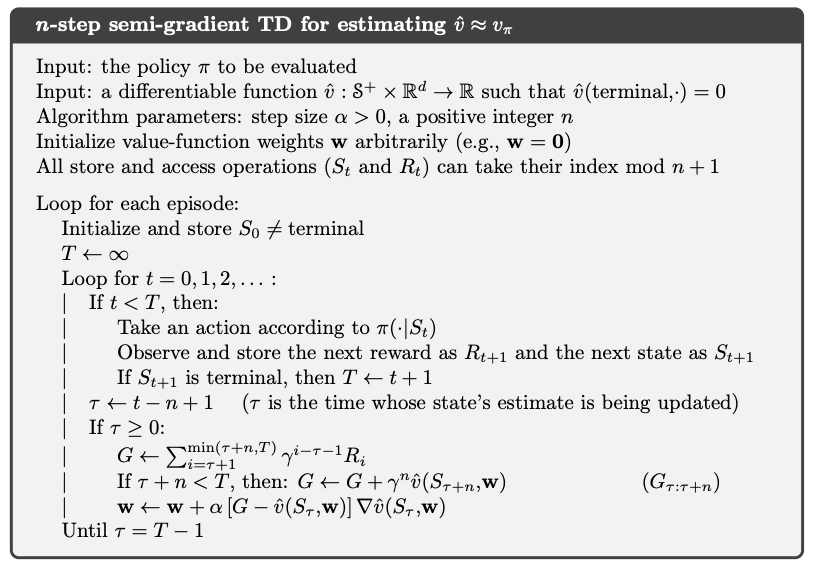
\includegraphics[width=0.8\textwidth]{/chapter9_1}
	\caption{Pseudocode for $n$-step semi-gradient TD for estimating $\hat{v} \approx v_\pi$}
	\label{fig: n-step algo}
\end{figure}

\subsection{Feature Construction for Linear Models}
Constructing features that are appropriate for the RL task is critical for providing the agent useful prior knowledge about the domain. In this section we will discuss different ways of constructing features.

\subsubsection{Polynomials}
We may want to design features with higher complexity than can be captured with linear methods. If we think of the example of parametrising a state $s$ by two dimensions $s_1 \in \mathbb{R}$ and $s_2 \in \mathbb{R}$, we could represent this state as $\textbf{x}(s) = (s_1, s_2)^T$. This, however, does not allow us to represent interactions between the two dimensions if they do indeed interact, and it would also mean that the value of our state would have to be 0 if both dimensions were zero. We can instead use a four-dimensional feature vector like: $\textbf{x}(s) = (1, s_1, s_2, s_1s_2)^T$. This allows us to capture any combination of these dimensions in polynomial space. The generalised form of polynomials is shown in Figure \ref{fig: poly}.

\begin{figure}
	\centering
	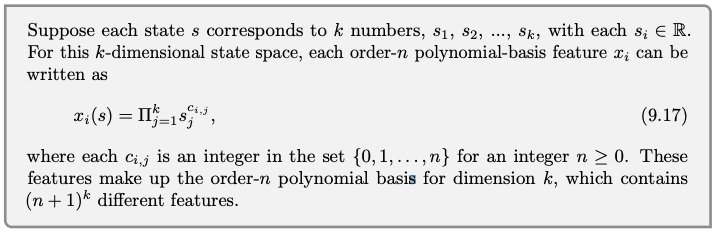
\includegraphics[width=0.8\textwidth]{/chapter9_2}
	\caption{Generalised form of polynomial basis}
	\label{fig: poly}
\end{figure}

Note that $c_{i,j}$ here is a matrix with $i$ rows corresponding to $i$ features and $j$ columns corresponding to $j$ dimensions.

\subsubsection{Fourier Basis}
Fourier series express periodic functions as weighted sums of sine and cosine basis functions (as features) of different frequencies, with a function $f$ being periodic if $f(x) = f(x + \tau)$ for all $x$ and some period $\tau$. The one-dimensional, order-$n$ Fourier cosine basis consists of the $n+1$ features:
\begin{equation}
	x_i(s) = cos(i\pi s), \; \; \; s \in [0,1]
\end{equation}
for $i = 0, \ldots, n$.

\subsubsection{Coarse Coding}
Consider a two dimensional state space represented by the set $s = \{s_1, s_2\}$. We can lay the state space out in two dimensions, and map circles to the state space as in Figure \ref{fig: coarse coding}. If one state $s$ falls within multiple overlapping circles, then another state covered by these circles $s'$ will be updated with the same value update. How we choose to define these circles (other indeed other shapes) defines the degree of generalisation across states. In effect, we are saying the states that lay close to each other in state space should be updated generally in proportion to one other.

\begin{figure}[h!]
	\centering
	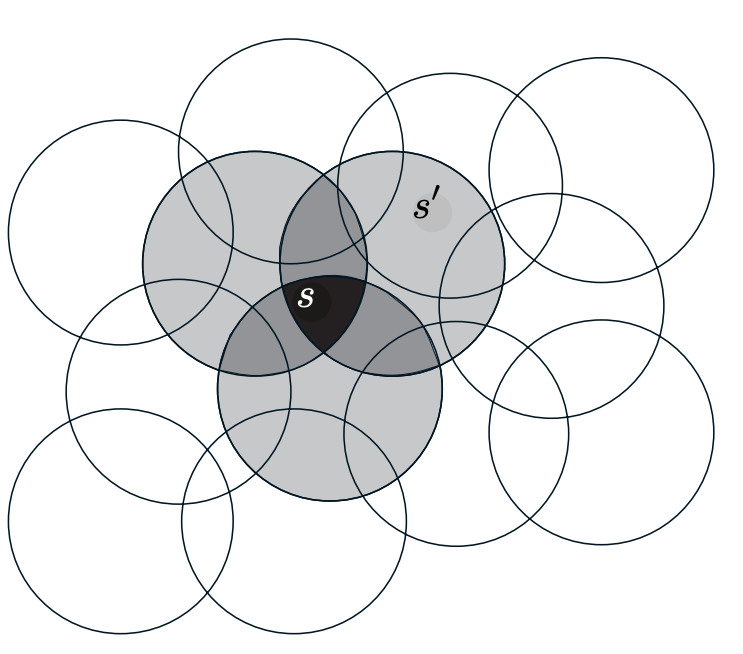
\includegraphics[width=0.75 \textwidth]{/chapter9_3}
	\caption{Coarse coding. Generalization from state $s$ to state $s_0$ depends on the number of their features whose receptive fields (in this case, circles) overlap. These states have one feature in common, so there will be slight generalization between them.}
	\label{fig: coarse coding}
\end{figure}

\subsubsection{Tile Coding}
Tile coding is similar to course coding, but now uses sets of overlapping, uniformly or asymmetrically distributed, tiles - Figure \ref{fig: tile coding}.  Tiles do not need to be squares, they can be irregular shapes, horizontal/vertical lines or log lines. Each affects the mode of generalisation in function approximation.

\begin{figure}[h!]
	\centering
	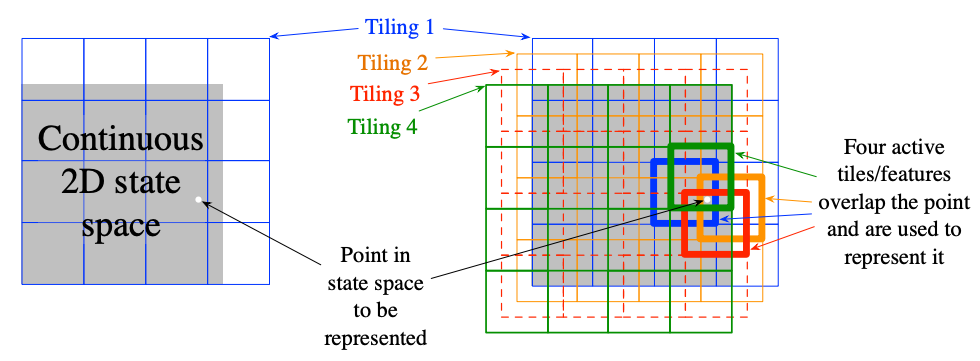
\includegraphics[width=\textwidth]{/chapter9_4}
	\caption{Multiple, overlapping grid-tilings on a limited two-dimensional space. These tilings are offset from one another by a uniform amount in each dimension.}
	\label{fig: tile coding}
\end{figure}

\subsubsection{Radial Basis Functions}
Radial Basis Functions (RBFs) are the natural extension of course coding to continuous-valued domains. Rather than a feature being either off or on (0 or 1), it can take any value in the interval [0,1]. Typical RBFs use Gaussian's to parametrise the distribution of the feature, which has centre state $c_i$ and width $\sigma_i$. The feature value therefore takes the form:
\begin{equation}
x_i(s) \doteq exp \left(-\frac{||s - c_i||^2}{2 \sigma_i^2}\right)
\end{equation}

Figure \ref{fig: rbf} shows the overlapping distribution of RBF features.

\begin{figure}[h!]
	\centering
	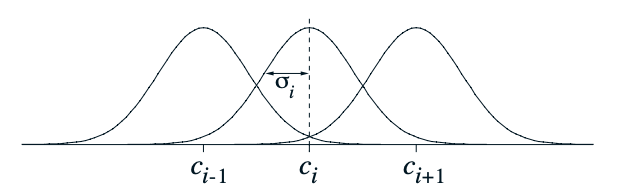
\includegraphics[width=0.75\textwidth]{/chapter9_5}
	\caption{One-dimensional radial basis functions.}
	\label{fig: rbf}
\end{figure}

\subsection{Selecting Step-Size Parameters Manually}
Can we say in general how best to select $\alpha$ in our function approximator? A good rule of thumb for setting the step-size parameter of linear SGD methods is:
\begin{equation}
	\alpha \doteq (\tau \mathbb{E}[\textbf{x}^T\textbf{x}])^{-1}
\end{equation}

where \textbf{x} is a random feature vector chosen from the same distribution as input vectors will be in the SGD, and $\tau$ is the number of experiences within which you would like to learn.

\subsection{Nonlinear Function Approximation: Artificial Neural Networks}
Artificial Neural Networks (ANNs) have proven to be some of the best non-linear function approximators. We know plenty about them already, so here is some general points:
\begin{itemize}
\item ANNs overfit on training data, a problem mitigated by dropout.
\item Batch normalization involves normalising the output of hidden layers before passing them to the next layer, and performing this process on mini-batches of data. This improves the learning rates of the algorithms.
\end{itemize}

\subsection{Least-Squares TD}
Earlier, we established the TD fixed point as
\begin{align}
\textbf{w}_{TD} &\doteq \textbf{A}^{-1}\textbf{b}
\end{align}
where
\begin{equation}
\textbf{b} \doteq \mathbb{E}[R_{t+1} \textbf{x}_t] \in \mathbb{R}^d \; \; \text{and} \; \; \textbf{A} \doteq \mathbb{E}\left[\textbf{x}_t(\textbf{x}_t - \gamma \textbf{x}_{t+1})^T\right] \in \mathbb{R}^{d \times d}
\end{equation}
Instead of computing this solution iteratively, we could compute estimates of $A$ and $b$ and then directly compute the TD fixed point– this is the Least Squares TD algorithm (LSTD). It forms the estimates:
\begin{equation}
\hat{\textbf{A}_t} \doteq \sum_{k=0}^{t-1} \textbf{x}_k(\textbf{x}_k - \gamma \textbf{x}_{k+1})^T + \epsilon \textbf{I} \; \; \text{and} \; \; \hat{\textbf{b}_t} \doteq \sum_{k=0}^{t-1} R_{k+1}\textbf{x}_k
\end{equation}

where $\textbf{I}$ is the identity matrix, and $\epsilon \textbf{I}$, for some small $\epsilon > 0$ ensures that $\hat{\textbf{A}_t}$ is always invertible. It looks like both $\hat{\textbf{A}_t}$ and $\hat{\textbf{b}_t}$ should be divided by $t$ to achieve the expectation, but the $t$s cancel when used to calculate the the TD fixed point as 
\begin{equation}
\textbf{w}_{TD} \doteq \hat{\textbf{A}^{-1}}\hat{\textbf{b}}
\end{equation}

The inversion of the matrix usually requires $O(d^3)$ computation, but can be done with $O(d^2)$ using the \textit{Sherman-Morrison formula}. LSTD's lack of step size parameter means it never forgets, which is sometimes desirable, but often not in RL problems where both the environment and policy change with time.

\subsection{Memory-based Function Approximation}
So far we have been parametrising functions that approximate our value function, and these parameters are updated as we see more data. These are examples of \textit{parametric} models. An alternative approach is to store examples of transitions or rewards from one state to the next, and querying them when we arrive in a state, similar to the approach used in Dyna - Chapter 8. These are \textit{nonparametric} models or \textit{memory-based} function approximators, with examples including nearest neighbours, or locally weighted regressions, with the weights being proportional to the distance between current state and queried state.

Because these methods are \textit{local} approximations rather than \textit{global}, they allow us to somewhat overcome the curse of dimensionality, and only approximate the value function where it is required, rather than across the entire state space. For example, if we are working with a state space with $k$ dimensions, a tabular method , storing a global approximation requires memory exponential in $k$, whereas storing examples in a memory-based method requires only memory proportional to $k$, or linear in the number of examples $n$.

\subsection{Kernel-based Function Approximation}
In the previous subsection, we discussed weighted average regression, where the weight is proportional to some measure of distance. The function that assigns the weights in often called the \textit{kernel function} or simply a \textit{kernel} and takes the form $k: \mathcal{S} \times \mathcal{S} \rightarrow \mathbb{R}$ and is summarised by $k(s, s')$. Viewed  slightly differently, $k(s, s')$ is a measure of the strength of generalization from $s'$ to $s$.

\textit{Kernel regression} is the memory-based method that computes a kernel weighted average of the targets of \textit{all} examples stored in memory, assigning the result to the query state. If $\mathbb{D}$ is the set of stored examples, and $g(s')$ denotes the target for state $s'$ in a stored example, then the value function is
\begin{equation}
\hat{v}(s, \mathcal{D}) = \sum_{s' \in \mathcal{D}} k(s, s')g(s')
\end{equation}

The common kernel is the Gaussian radial basis function (RBF) as defined earlier and in the Gaussian Process literature. Kernel based methods allow us to operate in the high-dimensional feature space, only using stored examples, and without needing a complex, parametrised model. This is the so-called \textit{kernel trick} and is the basis of many modern machine learning methods.

\subsection{Looking Deeper at On-policy Learning: Interest and Emphasis}
Until now we have treated all encountered states equally, but it is likely that we will actually be more interested in some states that others. To deal with this, we introduce two new concepts called \textit{interest} and \textit{emphasis}. Interest is the degree to which we value an accurate estimate of the value of a given state, generally $I_t \in [0,1]$ and emphasis in a scalar that multiplies the learning update and thus emphasises or de-emphasises the learning done at time $t$. The emphasis is determined recursively from the interest by
\begin{equation}
M_t = I_t + \gamma^n M_{t-n}
\end{equation}

\subsection{Key Takeaways}
\begin{itemize}
\item \textit{Generalization} of RL systems is critical to be applicable to artificial intelligence and large engineering problems. Generalization is achieved by approximating the value function using various techniques.
\item We defined the the prediction objective $\bar{VE}(\textbf{w})$, called the \textit{mean squared value error}, which provides a rational basis for comparing different function approximators.
\item Most techniques use stochastic gradient descent (SGD) to find the set of weight parameters than minimise $\bar{VE}(\textbf{w})$
\item Linear methods can be proven to converge to the globally optimum weight vector under certain conditions. 
\item Features, used to build linear methods, can take many forms, including: polynomials, fouriers, coarse codings, tile codings, and RBFs.
\item Artificial NNs have been proven to be potentially the most effective nonlinear function approximator.
\item Instead of using \textit{parametric} function approximators, \textit{non-parametric} models can be used that predict values based on the distance of a current state to past observed next states for which we have some stored values, or state representations.
\item \textit{Interest}and \textit{Emphasis} allow us to focus the function approximation on parts of the state space where we would value more accurate estimates.
\end{itemize}




